\section{Analisi}
La prima fase del processo di traduzione consta nell'eseguire l'analisi morfologica e sintattica della frase inserita dall'utente (Figura \ref{Vauquois_triangle}). \\
A tal fine, si è fatto uso delle API offerte dal progetto open-source Tint \cite{tint_due}.
Si sono sperimentate due modalità di interazione:
\begin{enumerate}
	\item Importazione libreria Java ed uso delle relative API\footnote{Per maggiori dettagli si rimanda il lettore alla sezione \textit{TINT Java API }della pagina: https://dh.fbk.eu/research/tint/download-and-usage/}
		\item Chiamata API REST al WebService di Tint, specificando nel body della richiesta HTTP la frase da processare.
		In Figura \ref{REST} viene mostrato come costruire la richiesta utilizzando l'applicativo Postman \footnote{Applicativo client utilizzabile per testare API REST (https://www.postman.com/)} ed il command line tool CURL\footnote{Strumento con interfaccia a riga di comando utilizzabile per trasferire dati attraverso la rete}. \\
		In questo modo si può dunque sviluppare applicativi di NLP senza essere legati all'utilizzo del linguaggio di programmazione Java, tuttavia i tempi di elaborazione possono essere influenzati dalla connessione di rete.
\end{enumerate}
	\begin{figure}[!ht]
	\centering
	\subcaptionbox{Client Postman}{%
		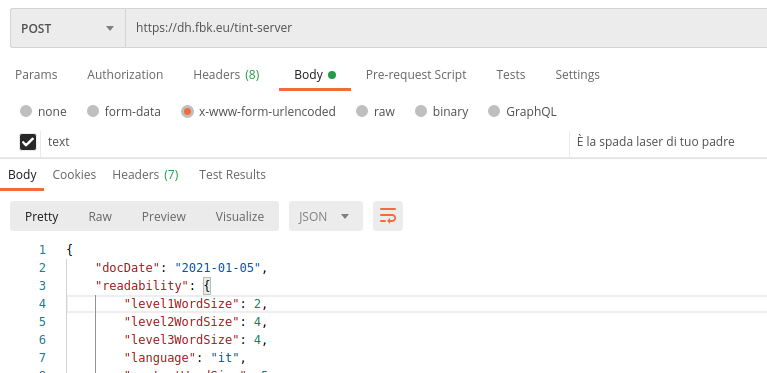
\includegraphics[width=0.75\textwidth]{./img/REST_Postman}%
	}\par\medskip
	\subcaptionbox{CURL}{%
		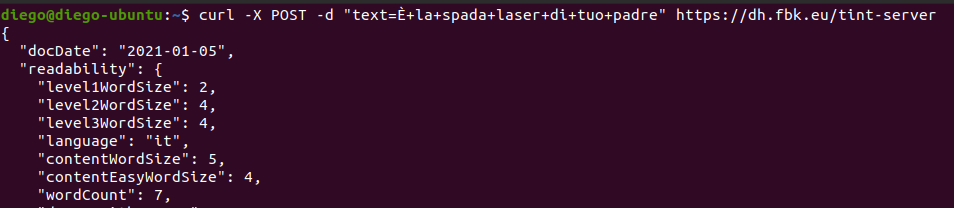
\includegraphics[width=0.75\textwidth]{./img/REST_CURL}%
	}
	\caption{Chiamata REST al server di Tint e successiva HTTP Response contenente dati in formato JSON}
	\label{REST}
\end{figure}
Indipendentemente dal tipo di interazione scelta, in entrambi i casi Tint restituisce in formato JSON il risultato della sua pipeline di elaborazione che comprende: segmentazione del testo in tokens, analisi morfologica ed individuazione dei morfemi, POS tagging, lemmatizzazione,  dependency parsing. \\
Analizzando il contenuto del JSON in questione, tra i vari dati è possibile notare la presenza di due JSONArray:
\begin{itemize}
	\item array "\textit{tokens}": 
	è il risultato della segmentazione del testo in \textbf{N tokens}\footnote{Nel seguito con le espressioni "parole della frase" o "elementi lessicali della frase" faremo riferimento ai suddetti tokens}.
	Ciascun elemento ha come attributi il lemma, il POS, l'insieme di morfermi, ... etc. Sono inoltre esplicitate in un sotto-array delle features linguistiche in relazione al valore del POS: genere e numero nel caso di un nome, tempo verbale nel caso di un verbo, ... etc.
	\item array "\textit{basic-dependencies}": è il risultato dell'analisi sintattica, più nello specifico del parsing a dipendenze. L'array contiene le \textbf{N-1 dipendenze}\footnote{Relazioni grammaticali binarie dirette tra gli elementi lessicali della frase.}, per ciascuna vengono specificati: 
		\begin{itemize}[label=$\ast$]
			\item indice $i\in[1,N]$ che punta alla parola della frase che funge da \textbf{testa}
			\item indice $j\in[1,N] \; (j \neq i) $ che punta alla parola che funge da \textbf{dipendente}
			\item etichetta della relazione
		\end{itemize}
	Nell'array è presente inoltre una relazione fittizia con etichetta "ROOT" che identifica la parola che costituisce la testa della frase (radice dell'albero).
\end{itemize}


Come verrà discusso nella Sezione {\ref{sec:transfer}}, nella fase di \textit{Transfer Sintattico} sarà necessario attraversare l'albero a dipendenze dalla radice verso le foglie, passando per i vari nodi intermedi.
Dato un nodo, dobbiamo disporre di opportuni puntatori che ci consentano di ottenere la lista dei nodi figli in tempo $\mathcal{O}(1)$ e di poter effettuare quindi la visita in ampiezza in tempo $\mathcal{O}(N)$;  cosa che risulterebbe impraticabile se utilizzassimo come struttura dati direttamente l'array \textit{basic-dependencies} di Tint (per ogni nodo visitato, l'insieme dei suoi figli sarebbero prelevati ogni volta in tempo $\mathcal{O}(N)$, un'ipotetica visita dell'albero in ampiezza richiederebbe quindi un tempo $\mathcal{O}(N^2)$). \\
Di conseguenza, a partire dall'array di relazioni di dipendenze sopra citato, viene costruita una struttura dati ad Albero con un numero arbitrario di figli (Figura \ref{tree}).
\begin{figure}[ht]
	\centering 
	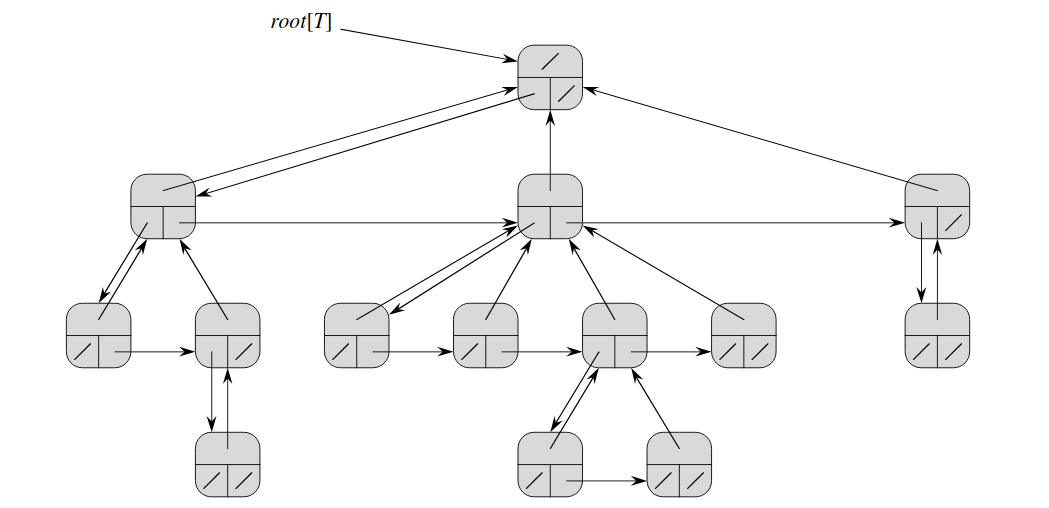
\includegraphics[scale=0.35]{./img/Albero}
	\caption{Rappresentazione intuitiva struttura dati ad albero.}
	\label{tree}
\end{figure}
\lstinputlisting[label={tree_code},style = javacode, caption ={Implentazione in Java struttura dati albero con numero arbitrario di figli. }]{java/Tree.java}
Nel Listing \ref{parsing_code} vengono riportati i dettagli relativi al processo di parsing e di generazione della struttura dati ad albero.
Ogni nodo dell'albero, corrispondente in maniera biunivoca ad una parola $i$ della frase, viene dotato di un puntatore "aggiuntivo" ad un oggetto di tipo \textit{MorphSyntaxInfo} che incapsula le informazioni morfologiche della parola in questione, provenienti dagli attributi dell'elemento $i$ dell'array "tokens" di Tint precedentemente descritto. 
Per ogni relazione di dipendenza, il nodo corrispondente al dipendente viene aggiunto alla lista dei figli del nodo corrispondente alla testa della relazione. \\
Al termine del processo restituiamo l'albero appena creato, che incorpora tutte le informazioni morfo-sintattiche della frase che potranno essere acquisite e processate visitando l'albero 
a partire dalla radice (testa della frase).



\lstinputlisting[label={parsing_code},style = javacode, caption ={Creazione \textbf{albero a dipendenze} a partire dalla frase in ingresso. }]{java/Parser.java}







%\item Vengono riconosciute solo le seguenti relazioni di dipendenza:
% \lstinputlisting[style = javacode, caption ={}]{java/deprel}
%\item I POS\footnote{acronimo di Part of Speech} riconosciuti ed analizzati sono esplicitati nella seguente enumerazione:
%\lstinputlisting[style = javacode, caption ={}]{java/pos}  